\documentclass[main.tex]{subfiles}
\begin{document}
\section{Приближаване с тръби}
\label{tubes}
В тази глава ще разгледаме в неголяма дълбочина построяване на модел с тръби. За повече подробности, може да се проследи подробното изложение в \cite{rabiner_schafer78} или по-сбитото в \cite{taylor:2009}.

За да извлечем спектралните свойства на вокалния тракт\footnote{както се зарекохме в предния раздел}, трябва да моделираме системата за производство на реч. Освен това искаме да можем да отделим характеристиките на вокалния тракт от тези на останалите части на системата. Един такъв модел се получава с модела на тръбите, който ще бъде описан в този раздел.

За улеснение, нека разгледаме конкретна конфигурация. Например тази, при произнасянето на фонемата ,,ъ'',тъй като е възможно най-проста. В този случай глотисът трепти, устата е отворена, а клапата към носната кухина е затворена.

Тъй като ,,ъ'' е гласна, което е озвучен тип звук, глотисът $g$ трепти псевдо-периодично, после вълната преминава и се променя от вокалния тракт $v$ и накрая излиза и се пречупва през устните $r$. Това означава, че ако глотисът има даден спектър, то вокалният тракт го променя (филтрира го), като усилва дадени честоти и заглушава други, до получаване на нов спектър. Устните допълнително филтрират спектъра. В крайна сметка получаваме нов сигнал, чийто спектър е резултат от умножението на спектрите на $g$, $v$ и $r$.

Тоест, ако $g \xleftrightarrow{\mathcal{F}\mathcal{S}} G(\mathcal{z}), v \xleftrightarrow{\mathcal{F}\mathcal{S}} V(\mathcal{z}), r \xleftrightarrow{\mathcal{F}\mathcal{S}} R(\mathcal{z})$, а новият сигнал е $y$ с $y \xleftrightarrow{\mathcal{F}\mathcal{S}} Y(\mathcal{z})$, е изпълнено, че

$\mathcal{Y}(\mathcal{z}) = \mathcal{G}(\mathcal{z}) \mathcal{V}(\mathcal{z}) \mathcal{R}(\mathcal{z})$,

където $\mathcal{z} = e^{i\omega_k}$ е прост сигнал с ъглова честота $\omega_k$, а $\xleftrightarrow{\mathcal{F}\mathcal{S}}$ обозначава Фурие преобразувание, което е въведено в \autoref{appendix:fourier}.\\

Във времевия домейн уравнението има вида $y(t) = g(t)\ast v(t)\ast r(t)$, както следва от \nameref{th:appendix:fourier:convolution} също в \autoref{appendix:fourier}.

Тъй като в крайна сметка получаваме нов сигнал при усните, това, от което се интересуваме, са спектралните особености на $\mathcal{V}(\mathcal{z})\mathcal{R}(\mathcal{z})$, за които можем да си мислим като един общ филтър, описващ вокалния тракт. За да говорим за крайния сигнал $\mathcal{Y}$, трябва да знаем какво е действието на входния сигнал $\mathcal{G}$, който ще бъде променян от филтъра на вокалния тракт. 

\begin{footnotesize}
    \textbf{Бележка:} Дефиницията за Фурие преобразувание изисква сингалът да е периодичен. В случая сме взели $g$ да е такъв. Нека засега приемем, че сигналите $v$ и $r$ също са периодични. Това, а също и че периодът им съвпада с този на $g$, е показано в $\autoref{systems:periodicity}$.
\end{footnotesize}

\begin{figure}[ht]%
    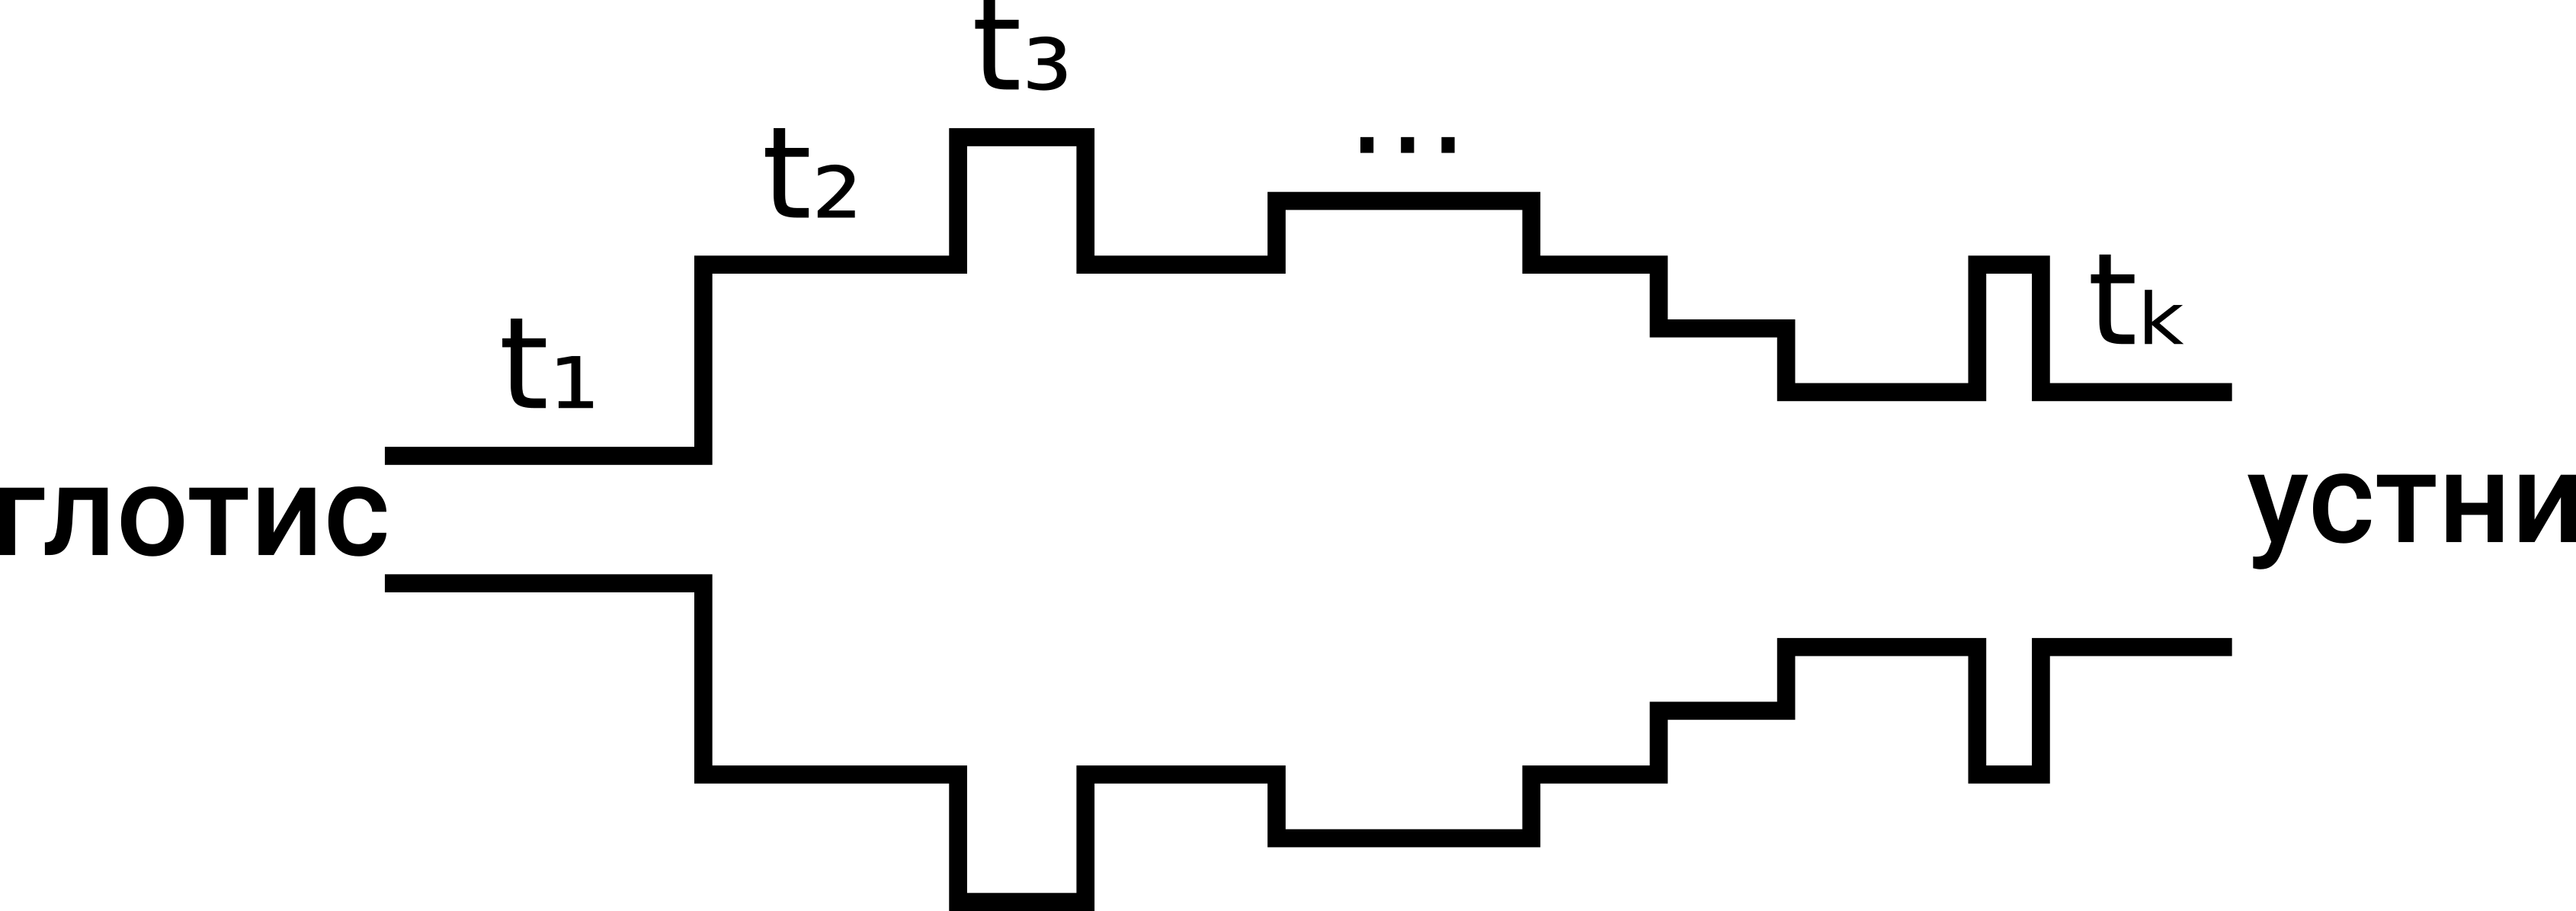
\includegraphics[width=\textwidth]{vocal_tubes}%
    \caption{Приближение на вокалния тракт с $N$ тръби}%
    \label{fig:tubes:1}
\end{figure}

Попринцип стените на вокалния тракт са гладки и меки, но това се моделира трудно. Допълнително, формата му е сложна и специфична за всеки човек. Така че нека опростим ситуацията, като използваме приближение с $N$ на брой тръби, номерирани $1...N$, с постоянно напречно сечение, както е показано на $\autoref{fig:tubes:1}$
За още по-голямо опростяване, нека няма и загуба на енергия, каквата би се получила попринцип.


Нека въведем следните стандартни означения:
\begin{enumerate}
    \item{$\mathcal{c}$} - скорост на звука в еластична среда
    \item{$\rho$} - плътност на въздуха в тръбите
    \item{$A$} - лицето на напречното сечение в тръба (константа)
    \item{$u = u(x, t)$} - е промяната в обемната скорост на позиция $x$ в момента $t$
    \item{$p = p(x, t)$} - е промяната в звуковото налягане
\end{enumerate}

Звуковите вълни, преминаващи през течна среда в
тръба, изпълняват уравнения:

\begin{subequations}
    \label{eq:tubes:01}
    \begin{flalign}
        \frac{\partial\rho}{\partial x} & = \frac{\rho}{A} \frac{\partial u}{\partial t}\\
        \frac{\partial u}{\partial x} & = \frac{A}{\rho \mathcal{c}^2} \frac{\partial \rho}{\partial t}
    \end{flalign}
\end{subequations}

и може да се покаже, че решенията на Уравнения \ref{eq:tubes:01} имат вида

\begin{subequations}
    \label{eq:tubes:02}
    \begin{flalign}
        \label{eq:tubes:02:a} u(x, t) & = \Q{u^+\B{t - \frac{x}{\mathcal{c}}} - u^-\B{t + \frac{x}{\mathcal{c}}}} && \\
        p(x, t) & = \cfrac{\rho \mathcal{c}}{A}\Q{p^+\B{t - \frac{x}{\mathcal{c}}} + p^-\B{t + \frac{x}{\mathcal{c}}}} &&
    \end{flalign}
\end{subequations}

Първо нека да разгледаме връзката между две съседни тръби.

\subsection{Преминаване от една тръба в друга}

Да разгледаме по-внимателно значението на $\eqref{eq:tubes:02:a}$.\\
При преминаване от една тръба в друга, част от вълните ще преминат към следващата тръба, а част от тях ще се отразят наобратно.
В такъв случай във всеки момент от време $t$ и във всяка точка $x$ на $k$-тата тръба, обемната скорост $u_k$ ще зависи от обемната скорост на вълните, които вървят ,,напред'' и тази на вълните, които вървят ,,назад''. За специфична тръба $k$, Уравнения $\eqref{eq:tubes:02}$ ще имат вида:

\begin{subequations}
    \label{eq:tubes:03}
    \begin{flalign}
        \label{eq:tubes:03:a} u_{k}(x, t) &= \Q{u_{k}^{+}\B{t - \cfrac{x}{\mathcal{c}}} - u_{k}^{-}\B{t + \cfrac{x}{\mathcal{c}}}} && \\
        p_{k}(x, t) &= \cfrac{\rho \mathcal{c}}{A_{k}} \Q{u_{k}^{+}\B{t - \cfrac{x}{\mathcal{c}}} + u_{k}^{-}\B{t + \cfrac{x}{\mathcal{c}}}},&&
    \end{flalign}
\end{subequations}

където $l_k$ е дължината, а $A_k$ е лицето на напречното сечение на $k$-тата тръба, $x$ е разстояние в нея ($0\leq x \leq l_k$), $t$ е момент от време.

Вълните, които вървят ,,напред'' и ,,назад'', ще означаваме съответно с $u^{+}$ и $u^{-}$.

Тъй като енергията трябва да се запази, въвеждаме допълнително условие за границата между две тръби:
\begin{subequations}
    \label{eq:tubes:04}
    \begin{flalign}
        u_k(l_k, t) & = u_{k+1}(0, t) &&\\
        p_k(l_k, t) & = p_{k+1}(0, t) &&
    \end{flalign}
\end{subequations}

Когато заместим Уравнения $\eqref{eq:tubes:04}$ в $\eqref{eq:tubes:03}$, получаваме:
\begin{flalign*}
    & u_k^+\B{t - \cfrac{l_k}{\mathcal{c}}} - u_k^{-}\B{t + \cfrac{l_k}{\mathcal{c}}} = u_{k+1}^{+}(t) - u_{k+1}^{-}(t) &&
    & \intertext{и}
    & \cfrac{\rho \mathcal{c}}{A_{k}} \Q{u_{k}^{+}\B{t - \cfrac{l_k}{\mathcal{c}}} + u_{k}^{-}\B{t + \cfrac{l_k}{\mathcal{c}}}} = \cfrac{\rho \mathcal{c}}{A_{k+1}} \Q{u_{k+1}^{+}(t) + u_{k+1}^{-}(t)} && \\
    & \iff && \\
    & \cfrac{A_{k+1}}{A_{k}}\Q{u_{k}^{+}\B{t - \cfrac{l_k}{\mathcal{c}}} + u_{k}^{-}\B{t + \cfrac{l_k}{\mathcal{c}}}} = u_{k+1}^{+}(t) + u_{k+1}^{-}(t) &&
\end{flalign*}


Нека означим с $\tau_{k}$ времето, за което вълна пропътува дължината на $k$-тата тръба, тоест $\tau_{k}= \cfrac{l_k}{\mathcal{c}}$. Тогава имаме:

\begin{flalign}
    \label{eq:tubes:05}
    & u_k^+(t - \tau_k) - u_k^{-}(t + \tau_k) = u_{k+1}^{+}(t) - u_{k+1}^{-}(t) && \\
    \label{eq:tubes:06}
    & \frac{A_{k+1}}{A_{k}}[u_{k}^{+}(t - \tau_k) + u_{k}^{-}(t + \tau_k)] = u_{k+1}^{+}(t) + u_{k+1}^{-}(t) &&
\end{flalign}

Първо, нека да изразим скоростта на вълните, които вървят "напред"
в $(k+1)$-та тръба $\B{u_{k+1}^{+}}$, чрез тези, които са преминали от предната тръба $\B{u_k^{+}}$
и тези, които се отразяват от текущата $\B{u_{k+1}^{-}}$.
\begin{flalign}
    & \nonumber \intertext{От $\eqref{eq:tubes:05}$ получаваме}
    & \label{eq:tubes:07} u_{k}^{-}(t + \tau_{k}) = u_{k}^{+}(t - \tau_k) - u_{k+1}^{+}(t)  + u_{k+1}^{-}(t) && \\
    & \nonumber \intertext{Заместваме $\eqref{eq:tubes:07}$ в $\eqref{eq:tubes:06}$}
    & \nonumber u_{k+1}^{+}(t) = \frac{A_{k+1}}{A_k} u_{k}^{+}(t - \tau_k) + \frac{A_{k+1}}{A_k}[u_{k}^{+}(t - \tau_k) - u_{k+1}^{+}(t)  + u_{k+1}^{-}(t)] - u_{k+1}^{-}(t)  && \\
    & \nonumber u_{k+1}^{+}(t)\Q{1 + \frac{A_{k+1}}{A_k}} = u_{k}^{+}(t - \tau_k)\frac{2A_{k+1}}{A_k} + u_{k+1}^{-}(t)\Q{\frac{A_{k+1}}{A_k} - 1}  && \\
    & \nonumber u_{k+1}^{+}(t)\Q{\frac{A_k + A_{k+1}}{A_k}} = u_{k}^{+}(t - \tau_k)\frac{2A_{k+1}}{A_k} + u_{k+1}^{-}(t)\Q{\frac{A_{k+1} - A_k}{A_k}} && \\
    & \label{eq:tubes:08} u_{k+1}^{+}(t) = u_{k}^{+}(t - \tau_k)\Q{\frac{2A_{k+1}}{A_k + A_{k+1}}} + u_{k+1}^{-}(t)\Q{\frac{A_{k+1} - A_k}{A_k + A_{k+1}}} &&
\end{flalign}

Коефициентът, който стои пред $u_k^{+}(t - \tau_k)$ в уравнение $\eqref{eq:tubes:08}$,
представлява количеството енергия, която преминава от тръба $k$ в тръба $k+1$,
идваща от вълните, които се движат "напред" в $k$-тата тръба. Затова
\begin{equation}
    \label{eq:tubes:09}
    t_k = \frac{2A_{k+1}}{A_k + A_{k+1}}
\end{equation}

се нарича \textbf{коефициент на преминаване} за $k$-тия преход (преходът между тръби $k$ и $k+1$).

Коефициентът пред $u_{k+1}^{-}(t)$ представлява количестото енергия, получена от вълните,
които вървят "назад" в тръба $k+1$. Затова 
\begin{equation}
    \label{eq:tubes:10}
    r_k = \frac{A_{k+1} - A_k}{A_k + A_{k+1}}
\end{equation}
се нарича \textbf{коефициент на отрязяване} за $k$-тия преход. 

Можем да забележим, че в специалния случай, в който напречните сечения на
две съседни тръби са равни ($A_k = A_{k+1}$), би следвало всички
вълни да преминават свободно. Наистина, ако заместим в уравнение $\eqref{eq:tubes:10}$,
$r_k = 0$, a от $\eqref{eq:tubes:09}$ се вижда, че $t_k = 1$

Нека изразим скоростта на вълните в тръба $k$ чрез скоростта на вълните в $(k+1)$-вата тръба. 
\begin{subequations}
    \label{eq:tubes:11}
    \begin{flalign}
        & \nonumber \intertext{Първо разместваме уравнение $\eqref{eq:tubes:08}$}
        &  u_k^{+}(t - \tau_k) = u_{k+1}^{+}(t)\Q{\frac{A_k + A_{k+1}}{2A_{k+1}}} + u_{k+1}^{-}(t)\Q{\frac{A_k - A_{k+1}}{2A_{k+1}}} \label{eq:tubes:11:a} && \\
        & \nonumber \intertext{Заместваме $\eqref{eq:tubes:11:a}$ в $\eqref{eq:tubes:05}$}
        & \nonumber u_k^{-}(t + \tau_k) = u_k^{+}(t - \tau_k) - u_{k+1}^{+}(t) + u_{k+1}^{-}(t) && \\
        & \nonumber u_k^{-}(t + \tau_k) = u_{k+1}^{+}(t)\Q{\frac{A_k + A_{k+1}}{2A_{k+1}}} + u_{k+1}^{-}(t)\Q{\frac{A_k - A_{k+1}}{2A_{k+1}}} - u_{k+1}^{+}(t) + u_{k+1}^{-}(t) && \\
        & \nonumber u_k^{-}(t + \tau_k) = u_{k+1}^{+}(t)\Q{\frac{A_k + A_{k+1} - 2A_{k+1}}{2A_{k+1}}} + u_{k+1}^{-}(t)\Q{\frac{A_k - A_{k+1} + 2A_{k+1}}{2A_{k+1}}} && \\
        & \label{eq:tubes:11:b} u_k^{-}(t + \tau_k) = u_{k+1}^{+}(t)\Q{\frac{A_k - A_{k+1}}{2A_{k+1}}} + u_{k+1}^{-}(t)\Q{\frac{A_k + A_{k+1}}{2A_{k+1}}} &&
    \end{flalign}
\end{subequations}

Използвайки, че
\begin{flalign*}
    \cfrac{1}{1 + r_k} & = \cfrac{A_k + A_{k+1}}{A_{k+1} - A_k + A_{k+1} + A_k} = \cfrac{A_k + A_{k+1}}{2A_{k+1}} && \\
    \\
    \cfrac{r_k}{1 + r_k} & = \cfrac{(A_{k+1} - A_k)}{(A_k + A_{k+1})} \cfrac{(A_k + A_{k+1})}{2A_{k+1}} = \cfrac{A_{k+1} - A_k}{2A_{k+1}}, &&
\end{flalign*}
можем да запишем Уравнения $\eqref{eq:tubes:11}$ във вида:

\begin{subequations}
    \label{eq:tubes:12}
    \begin{flalign}
       & u_k^{+}(t - \tau_k) = \cfrac{1}{1 + r_k} u_{k+1}^{+}(t) - \cfrac{r_k}{1+r_k} u_{k+1}^{-}(t) && \\
       & u_k^{-}(t + \tau_k) = - \cfrac{r_k}{1+r_k} u_{k+1}^{-}(t) + u_{k+1}^{+}(t) + \cfrac{1}{1 + r_k} u_{k+1}^{-}(t) &&
    \end{flalign}
\end{subequations}

Сега да разгледаме Уравнения $\eqref{eq:tubes:12}$ в честотния домейн. Избираме $\mathcal{z} = e^{i\omega_k}$ и използваме свойствата, описани в \autoref{appendix:fourier}. Тоест, че $u_k[t - \tau_k] \xleftrightarrow{\mathcal{F}\mathcal{S}} \mathcal{z}^{-\tau_k}U_k(\mathcal{z})$
\begin{subequations}
    \label{eq:tubes:13}
    \begin{flalign}
        & \nonumber \mathcal{z}^{-\tau_k}U_k^{+}(\mathcal{z}) = \cfrac{1}{1 + r_k} U_{k+1}^{+}(\mathcal{z}) - \cfrac{r_k}{1+r_k} U_{k+1}^{-}(\mathcal{z}) && \\
        & \nonumber \mathcal{z}^{\tau_k} U_k^{-}(\mathcal{z}) = - \cfrac{r_k}{1+r_k} U_{k+1}^{-}(\mathcal{z}) + U_{k+1}^{+}(\mathcal{z}) + \cfrac{1}{1 + r_k} U_{k+1}^{-}(\mathcal{z}) && \\
        & \iff && \\
        & U_k^{+}(\mathcal{z}) = \cfrac{\mathcal{z}^{\tau_k}}{1 + r_k} U_{k+1}^{+}(\mathcal{z}) - \cfrac{r_k\mathcal{z}^{\tau_k}}{1+r_k} U_{k+1}^{-}(\mathcal{z}) && \\
        & U_k^{-}(\mathcal{z}) = - \cfrac{r_k\mathcal{z}^{-\tau_k} }{1+r_k} U_{k+1}^{-}(\mathcal{z}) + U_{k+1}^{+}(\mathcal{z}) + \cfrac{\mathcal{z}^{-\tau_k} }{1 + r_k} U_{k+1}^{-}(\mathcal{z}) &&
    \end{flalign}
\end{subequations}

По този начин получихме връзката между две съседни тръби. За да получим общия модел, трябва да отчетем двете специални ситуации - при първата и при последната тръба.

\subsection{Ограничения при устните}\label{tubes:lips}
%why you do this%

 	᠎
 	᠎ 
%mongolian vowel separator%

\begin{center}
\begin{figure}[ht]%
    \centering
    \begin{changemargin}{0cm}{0cm} 
        \subfloat[Представяне на устните като отвор в сферична преграда]{%
            \label{fig:tubes:3:a}
            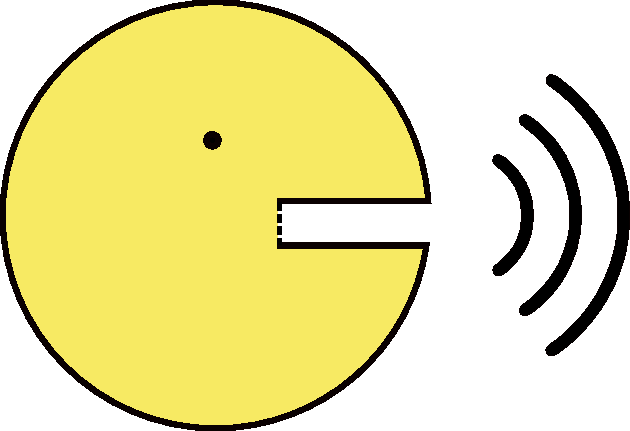
\includegraphics[height=10em,valign=t]{lips_a}%
        } 
        \hspace{0.2\paperwidth}
        \subfloat[Представяне на устните като отвор в безкрайна равнина]{%
            \label{fig:tubes:3:b}
            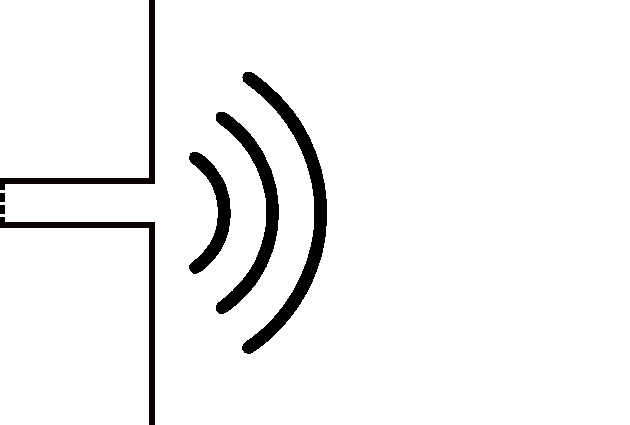
\includegraphics[height=10em,valign=t]{lips_b}%
        }
    \end{changemargin} 
    \caption{Представяне на устните като отвор в преграда}%
    \label{fig:tubes:3}
\end{figure}
\end{center}

Един разумен начин да представим изхода при устните е показан на Фигура \autoref{fig:tubes:3:a}. На фигурата се вижда как звуковите вълни, които напускат системата, претърпяват дифракция при отвора в сферичната повърхност, моделираща главата. Представянето на тази дифракция е сложно, затова ще се опитаме да го опростим.

Ако отворът на устните е много малък спрямо размера на сферата, то можем да 
си мислим за преградата като за безкрайна равнина, както е показано на Фигура \autoref{fig:tubes:3:b}

В такъв случай може да се покаже, че съществува следната връзка между налягането и обемната скорост:
\begin{equation}
    \label{eq:tubes:14}
    \mathcal{P}_N(l_N, \mathcal{z}) = Z_L(\mathcal{z}) \mathcal{U}_N(l_N, \mathcal{z}),
\end{equation}
където 
$Z_L(\mathcal{z})$ се нарича радиационен импеданс (пълно съпротивление), описва загубите, които се получават на изхода, и има вида:
\begin{align}
    \label{eq:tubes:impedance}
    Z_L(\mathcal{z}) = \cfrac{i\mathcal{z} L_r R_r}{R_r + i\mathcal{z} L_r},    
\end{align}
Където $\mathcal{z} = e^{i\omega_k}$ описва сигнал с ъглова честота $\omega_k$, $L_r$ и $R_r$ са константи, определени от размера на отвора на устата. За практически цели се избират:

\begin{multicols}{2}
    \begin{equation*}
      R_r = \cfrac{128}{9\pi^2} > 1
    \end{equation*}\break
    \begin{equation*}
      L_r = \cfrac{8a}{3\pi \mathcal{c}}
    \end{equation*}
  \end{multicols}
$a$ - радиус на отвора, $\mathcal{c}$ - скоростта на звука.

При много ниски честоти $Z_L(\mathcal{z}) \approx 0$, което значи, че съпротивлението на устните е почти нулево.
При средни честоти ($\mathcal{z}L_r \ll R_r$), $Z_L(\mathcal{z}) \approx i\mathcal{z}L_r$, а високи честоти, ($\mathcal{z}L_r \gg R_r$) $Z_L(\mathcal{z}) \approx R_r$. 
Това значи, че загубите при устните са най-големи при големи честоти, тъй като тогава импедансът е най-голям.

В случая, в който честотата $\mathcal{z}$ е висока, $Z_L \approx R_r$ е реално число  и не зависи от $\mathcal{z}$, тоест $Z_L(\mathcal{z}) = Z_L$. 

Тогава, ако $p_N(l_N, t)  \xleftrightarrow{\mathcal{F}\mathcal{S}}  P_N(l_N, \mathcal{z}), u_N(l_N, t) \xleftrightarrow{\mathcal{F}\mathcal{S}} U_N(l_N, \mathcal{z}) \text{ и съответно } Z_L \xleftrightarrow{\mathcal{F}\mathcal{S}} Z_L$, можем да разгледаме уравнението $\eqref{eq:tubes:14}$ във
времевия домейн:
\begin{flalign*}
    & p_N(l_N, t) = Z_L u_N(l_N, t), &&
\end{flalign*}

Ако използваме Уравнения \eqref{eq:tubes:03} и заместим с $\tau_N = \frac{l_N}{\mathcal{c}}$, получаваме:
\begin{flalign}
    & \nonumber \cfrac{\rho\mathcal{c}}{A_N}\Q{u_N^{+}(t - \tau_N) + u_N^{-}(t + \tau_N)} = Z_L\Q{u_N^{+}(t - \tau_N) - u_N^{-}(t + \tau_N)} &&\\
    & \nonumber u_N^{-}(t + \tau_N) \cfrac{(\rho\mathcal{c} + A_N Z_L)}{A_N} = u_N^{+}(t - \tau_N) \cfrac{(A_N Z_L - \rho\mathcal{c})}{A_N} &&\\
    & \label{eq:tubes:15} u_N^{-}(t + \tau_N) = -r_L u_N^{+}(t - \tau_N), \text{ където}&&
\end{flalign}

\begin{align*}
    r_L = \B{\frac{\frac{\rho\mathcal{c}}{Z_L} - A_N}{\frac{\rho\mathcal{c}}{Z_L} + A_N}}
\end{align*}

В случая, в който $Z_L \approx i\mathcal{z}L_r$ е комплексно, може да се покаже, че уравнение \eqref{eq:tubes:15} остава в сила,
но в този случай и $r_L$ също ще бъде комплексно.

\subsection{Ограничения при глотиса}

Както при устните, така и при глотиса, трябва да се отчете импедансът. Например когато глотисът е затворен, импедансът е безкраен, а обемната скорост нулева.

Връзката $U_1(0, \mathcal{z}) = U_G(\mathcal{z})$ е твърде наивна и може да се покаже, че по-добро приближение би било:
\begin{align}
\label{eq:tubes:16}
    U_1(0, \mathcal{z}) =  U_G(\mathcal{z}) - \frac{P_1(0, \mathcal{z})}{Z_G(\mathcal{z})},
\end{align}
където $\mathcal{z} = e^{i\omega_k}$, $Z_G$ описва импеднса на глотиса и $Z_G(\mathcal{z}) = R_G + i \mathcal{z} L_G,$

$L_G, R_G$ - константи
Отново предполагайки, че $Z_G$ е реално, тоест честотата $\omega_k$ е много ниска, можем да разгледаме
уравнение $\eqref{eq:tubes:16}$ във времевия домейн.

Нека $u_1(0, t)  \xleftrightarrow{\mathcal{F}\mathcal{S}} U_1(0, \mathcal{z}), p_1(0, t) = \xleftrightarrow{\mathcal{F}\mathcal{S}} P_q(0, \mathcal{z})$ за фиксиран първи аргумент и съответно $Z_G \xleftrightarrow{\mathcal{F}\mathcal{S}} Z_G$:

\begin{flalign*}
    & u_1(0, t) = u_G(t) - \cfrac{p_1(0, t)}{Z_G} &&
\end{flalign*}

Ако използваме Уравнения \eqref{eq:tubes:03}, получаваме

\begin{flalign*}
    & u_1^{+}(t) - u_1^{-}(t) = u_G(t) - \frac{\rho \mathcal{c}}{A_1}\Q{\frac{u_1^{+}(t) + u_1^{-}(t)}{Z_G}} && \\
    & u_1^{+}(t)\Q{1 + \frac{\rho\mathcal{c}}{A_1 Z_G}}  = u_G(t) + u_1^{-}(t)\Q{1 - \frac{\rho\mathcal{c}}{A_1 Z_G}} && \\
    & u_1^{+}(t) = u_G(t)\Q{\frac{A_1 Z_G}{A_1 Z_G + \rho \mathcal{c}}} + u_1^{-}(t)\Q{\frac{A_1 Z_G - \rho \mathcal{c}}{A_1 Z_G + \rho \mathcal{c}}} &&\\
\end{flalign*}
\begin{flalign}
    \label{eq:tubes:17}
    & u_1^{+}(t) = u_G(t) \Q{\frac{1 + r_G}{2}} + r_G u_1^{-}(t)&&
\end{flalign}

където $r_G = \B{\cfrac{A_1 Z_G - \rho\mathcal{c}}{A_1 Z_G + \rho\mathcal{c}}}$
и е изпълнено
\begin{flalign*}
    \cfrac{1 + r_G}{2} & = \cfrac{A_1Z_G + \rho\mathcal{c} + A_1Z_G - \rho\mathcal{c}}{2(A_1Z_G + \rho\mathcal{c})} = \cfrac{A_1Z_G}{A_1Z_G + \rho\mathcal{c}} && \\
\end{flalign*}

Ако се върнем в честотния домейн:
\begin{flalign}
    \label{eq:tubes:18}
    & U_G(\mathcal{z}) = \Q{\frac{2}{1 + r_G}}U_1^{+}(\mathcal{z}) - \Q{\frac{2r_G}{1 + r_G}}U_1^{-}(\mathcal{z}), &&
\end{flalign}


Отново може да се покаже, че ако $Z_G$ е комплексно, уравнението $\eqref{eq:tubes:17}$ е в сила и
в този случай $r_G$ също е комплексно.
За улеснение обикновено $Z_L$ и $Z_G$ се взимат реални. 

\subsection{Общ вид на $\mathcal{V}$}
За да видим общия вид на $\mathcal{V}$, нека засега всички тръби имат равна дължина и тя е $\tau_i = \frac{1}{2}, i \in[1...N]$
Тогава уравнения $\eqref{eq:tubes:13}$ имат вида:

\begin{subequations}
    \label{eq:tubes:19}
    \begin{flalign}
        & U_k^{+}(\mathcal{z}) = \cfrac{\mathcal{z}^{1/2}}{1 + r_k} U_{k+1}^{+}(\mathcal{z}) - \cfrac{r_k\mathcal{z}^{1/2}}{1+r_k} U_{k+1}^{-}(\mathcal{z}) &&\\
        & \nonumber \\
        & U_k^{-}(\mathcal{z}) = - \cfrac{r_k\mathcal{z}^{-1/2} }{1+r_k} U_{k+1}^{-}(\mathcal{z}) + U_{k+1}^{+}(\mathcal{z}) + \cfrac{\mathcal{z}^{-1/2} }{1 + r_k} U_{k+1}^{-}(\mathcal{z}) &&
    \end{flalign}
\end{subequations}

За да опишем граничните условия при устните, дефинираме $U_{N+1}(\mathcal{z})$ да е Фурие трансформацията
на входа на несъществуваща $(N+1)$ тръба. Тази тръба е безкрайно дълга и заради това скоростта на вървящите ,,назад'' вълни трябва да бъде 0

Тоест дефинираме:
\begin{flalign}
    \label{eq:tubes:20}
    & U_{N+1}^{+} (\mathcal{z}) = U_L(\mathcal{z}) &&\\
    & \nonumber U_{N+1}^{-}(\mathcal{z}) = 0 &&
\end{flalign}

Също така искаме коефициентът на отражение на последната истинска тръба да е равен на коефициент на отражение при устните, а именно $r_N = r_L$
\begin{flalign*}
    & \B{\frac{A_{N+1} - A_N}{A_{N+1} + A_N}} = \B{\frac{\frac{\rho\mathcal{c}}{Z_L} - A_N}{\frac{\rho\mathcal{c}}{Z_L} + A_N}} &&
\end{flalign*}

Това ни дава, че $A_{N+1} = \frac{\rho\mathcal{c}}{Z_L}$

Ако представим Уравнения $\eqref{eq:tubes:19}$ в матричен вид, получаваме:

$U_k = Q_k U_{k+1}$ за

\begin{multicols}{2}
    $U_k = 
        \begin{bmatrix}
            U_k^{+}(\mathcal{z}) \\
            U_k^{-}(\mathcal{z}) \\
        \end{bmatrix}$
    \vfill
    \columnbreak
    $Q_k = 
        \begin{bmatrix}
            \cfrac{\mathcal{z}^{1/2}}{1 + r_k} & \cfrac{-r_k \mathcal{z}^{1/2}}{1 + r_k} \\
            & \\
            \cfrac{-r_k \mathcal{z}^{-1/2}}{1 + r_k} & \cfrac{\mathcal{z}^{-1/2}}{1 + r_k} \\
        \end{bmatrix}$
\end{multicols}

\begin{flalign*}
    & U_1 = Q_1 U_2 = Q_1 Q_2 U_3 = \cdots = Q_1 ... Q_N U_{N+1} = \Q{\prod_{i=1}^{N} {Q_i}}U_{N+1} &&
\end{flalign*}

За специалното ограничение глотиса, разгледаме матричния вид на $\autoref{eq:tubes:18}$
\begin{flalign*}
    & U_G(\mathcal{z}) = \left[
        \begin{array}{cc}
            \cfrac{2}{1+r_G}, & -\cfrac{2r_G}{1 + r_G} \\
        \end{array}
    \right] U_1 &&
\end{flalign*}

Ограниченията $\eqref{eq:tubes:20}$ за $U_L$ ни дават, че

\begin{flalign*}
    & U_{N+1} = 
    \left[ \begin{array}{cc}
            U_{N+1}^{+}(\mathcal{z}) \\
            U_{N+1} ^{-}(\mathcal{z})
        \end{array}\right] = 
    \left[ \begin{array}{cc}
        U_L(\mathcal{z}) \\
        0
    \end{array}\right]= 
    \left[ \begin{array}{cc}
        1 \\
        0
    \end{array}\right] U_L(\mathcal{z}) && \\ 
\end{flalign*}

Тогава, ако заместим, получаваме:

\begin{flalign}
    \label{eq:tubes:21}
    \nonumber \frac{1}{\mathcal{V}(\mathcal{z})} & = \frac{U_G(\mathcal{z})}{U_L(\mathcal{z})}  = \cfrac{\left[
        \begin{array}{cc}
            \cfrac{2}{1+r_G}, & -\cfrac{2r_G}{1 + r_G} \\
        \end{array}
        \right] \prod_{i=1}^{N} {Q_i} \left[ \begin{array}{cc}
            1 \\
            0
        \end{array}\right]U_L(\mathcal{z})}{U_L(\mathcal{z})} = && \\
        \nonumber \\
        & = \left[
            \begin{array}{cc}
                \cfrac{2}{1+r_G}, & -\cfrac{2r_G}{1 + r_G} \\
            \end{array}
            \right] \prod_{i=1}^{N} {Q_i} \left[ \begin{array}{cc}
                1 \\
                0
            \end{array}\right] &&
\end{flalign}
        

Нека изразим $Q_k$ по следния начин:

\begin{flalign*}
    & Q_k = \left[\begin{array}{cc}
            \cfrac{\mathcal{z}^{1/2}}{1 + r_k} & \cfrac{-r_k \mathcal{z}^{1/2}}{1 + r_k} \\
            & \\
            \cfrac{-r_k \mathcal{z}^{-1/2}}{1 + r_k} & \cfrac{\mathcal{z}^{-1/2}}{1 + r_k} \\
        \end{array}\right] = 
        z^{1/2}\left[\begin{array}{cc}
            \cfrac{1}{1 + r_k} & \cfrac{-r_k}{1 + r_k} \\
            & \\
            \cfrac{-r_k \mathcal{z}^{-1}}{1 + r_k} & \cfrac{\mathcal{z}^{-1}}{1 + r_k} \\
        \end{array}\right] = 
        \mathcal{z}^{1/2} \hat{Q}_k && 
\end{flalign*}

Тогава уравнение $\eqref{eq:tubes:21}$ има вида


\begin{flalign}
    \label{eq:tubes:22}
    & \frac{1}{\mathcal{V}(\mathcal{z})} = \frac{U_G(\mathcal{z})}{U_L(\mathcal{z})}  = \mathcal{z}^{N/2}\left[
        \begin{array}{cc}
            \cfrac{2}{1+r_G}, & -\cfrac{2r_G}{1 + r_G} \\
        \end{array}
        \right] \prod_{i=1}^{N} {\hat{Q}_i} \left[ \begin{array}{cc}
            1 \\
            0
        \end{array}\right] &&
\end{flalign}
        
Нека изразим общия вид на $\mathcal{V}(\mathcal{z})$. За $N=2$, например, има вида:

\begin{flalign}
\label{eq:tubes:23}
& \mathcal{V}(\mathcal{z}) = \frac{0.5 (1+r_G)\prod\limits_{i=1}^{2}(1 + r_i)\mathcal{z}^{-1}}{1 + (r_Gr_1 + r_1r_2)\mathcal{z}^{-1} + (r_Gr_2)\mathcal{z}^{-2}}, &&
\end{flalign}
както е показано в $\autoref{appendix:2:02}$

Може да се покаже, че в общия случай за произволно $N$, \autoref{eq:tubes:22} може да се развие итеративно до:

\begin{align}
    \label{eq:tubes:24}
    \mathcal{V}(\mathcal{z}) = \frac{0.5(1+r_G)\prod\limits_{i=1}^{N}{(1 + r_i)} \mathcal{z}^{-N/2}}{1 - \sum\limits_{i=1}^{N}{\alpha_i \mathcal{z}^{-i}}}
\end{align}

Както се вижда от $\autoref{appendix:2:01}$, предположението, че $\tau_i = \frac{1}{2}$ е разумно, тъй като при тази стойност се получава наи-голяма изразителна сила, както е отбелязано и в \hyperref[can:i]{Бележката}.

%============================================================================
\subsection{Общ вид на $\mathcal{R}$}

Моделът, описан в \autoref{tubes:lips} се моделира прекалено трудно. Може да се покаже (\cite{taylor:2009},\cite{quatieri}) , че ефектът от радиацията
се приближава достатъчно добре с една нула в единичната окръжност, тоест:
\begin{flalign}
    \label{eq:tubes:25}
    & \mathcal{R}(\mathcal{z}) = (1 - \gamma\mathcal{z} ^ {-1}) &&
\end{flalign}

%============================================================================
\subsection{Общ вид на $\mathcal{G}$}

За да се симулира действието на глотиса, трябва да отчетем как се държи той при
изговаряне на различни видове звуци. 

\begin{figure}[ht]%
    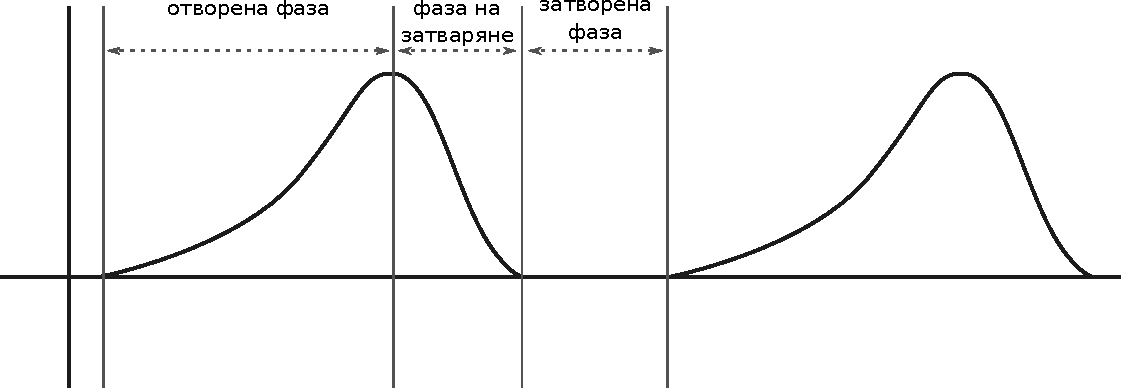
\includegraphics[width=\textwidth]{glotal_pulse}%
    \caption{Пример за импулс от глотиса}%
    \label{fig:tubes:2}
\end{figure}

В случая на гласна, както бяхме приели за улеснение, той трепти периодино и видът му може да се види на \autoref{fig:tubes:2}.
Можем да разделим този сигнал на три фази:

\begin{enumerate}
    \item Отворена фаза с край $F_1$
    \item Фаза на затваряне с начало $F_1$ и край $F_2$
    \item Затворена фаза с начало $F_2$
\end{enumerate}

Това може да се опише като функция на времето по следния начин.

\begin{flalign*}
    & g(t) = 
    \begin{cases}
        \cfrac{1}{2}( 1 - \cos{(\pi n / F1)}), & 0\leq t \leq F_1\\
        \cos{(\pi(n - N_1)/2N_2)}, & F_1 \leq t \leq F_2\\
        0, & \text{иначе}   
    \end{cases}   &&     
\end{flalign*}

Поведението като това на $\mathcal{G}$ може да се приближава с два полюса, както е показано в \nameref{appendix:poles}, тоест
\begin{flalign*}
    & \tilde{\mathcal{G}}(\mathcal{z}) = \cfrac{1}{(1-\alpha_1\mathcal{z}^{-1})(1 - \beta\mathcal{z}^{-1})}&&
\end{flalign*}
но по този начин не се отчита правилно самата форма на сигнала.

В \cite{quatieri}
е показано, че по-добро приближение се получава при $\alpha = \beta$ и $\mathcal{G}(\mathcal{z}) = \tilde{\mathcal{G}}(-\mathcal{z})$, тоест
\begin{flalign*}
    & \mathcal{G}(\mathcal{z}) = \frac{1}{(1 - \beta\mathcal{z})^2}&&
\end{flalign*}

Сигналът, показан на \autoref{fig:tubes:2}, е почти идеален. В действителност е почти невъзможно да се поддържа тон, който има еднакви разстояния между
пиковете и еднаква амплитуда. Отклонението от истинския период се нарича джитер\footnote{На английски jitter, думата е заемка, тъй като няма друг възприет български термин. Руският термин е джиттер}. Другият ефект, който е важен за истинския човешки глас, е трептенето\footnote{На английски shimmer. Тук също не мога да намеря подходящ български термин, но в случая и единственият руски, който открих, е шиммер}, тоест разликата в амплитудите. Освен за естествеността на гласа, тези характеристики могат да носят информация и за емоционалното състояние. Висок джитер може да означава дрезгав глас, но също може да се предизвика при чувство на стрес или страх.
Включването им в модела се постига с допълнителни нули, което ни дава и крайния видна $\mathcal{G}$ в случая на озвучен звук:

\begin{align}
    \label{eq:tubes:26}
    \mathcal{G}(\mathcal{z}) = \frac{\prod\limits_{i=0}^K (1 - \beta_i \mathcal{z}^{-1})}{(1 - \beta\mathcal{z})^2}
\end{align}

Да разгледаме случая с беззвучен звук. При съгласните, например, сигналът от глотиса е случайна редица с плосък спектър (тоест има почти еднаква мощност в целия спектър). Добър начин да се моделира е чрез генератор на бял шум.

\subsection{Общ вид на $\mathcal{Y}$}
От уравнения $\ref{eq:tubes:24}, \ref{eq:tubes:25}, \ref{eq:tubes:26}$ следва, че видът на  $\mathcal{H}$ е
\begin{flalign*}
    & \mathcal{Y}(\mathcal{z}) = \mathcal{G}(\mathcal{z})\mathcal{V}(\mathcal{z})\mathcal{R}(\mathcal{z}) = \Q{\frac{\prod\limits_{i=0}^K (1 - \beta_i \mathcal{z}^{-1})}{(1 - \beta\mathcal{z})^2}} \Q{\frac{0.5(1+r_G)\prod\limits_{i=1}^{N}{(1 + r_i)} \mathcal{z}^{-N/2}}{1 - \sum\limits_{i=1}^{N}{\alpha_i \mathcal{z}^{-i}}}} \Q{(1 - \gamma\mathcal{z} ^ {-1})}  &&
\end{flalign*}

При определени стойности на коефициентите, видът на $\mathcal{Y}$ може да се запише като:

\begin{flalign}
    \label{eq:tubes:27}
    & \mathcal{Y}(\mathcal{z}) = \mathcal{G}(\mathcal{z}) \cfrac{\sum\limits_{m=0}^{M} b_m \mathcal{z}^{-m} }{\sum\limits_{k=0}^{K} a_k \mathcal{z}^{-k}}, &&
\end{flalign}

от което ще се възползваме в следващия раздел.

\end{document}